%%%%%%%%%%%%%%%%%%%%%%%%%%%%%%%%%%%%%%%%%
% Beamer Presentation
% LaTeX Template
% Version 1.0 (10/11/12)
%
% This template has been downloaded from:
% http://www.LaTeXTemplates.com
%
% License:
% CC BY-NC-SA 3.0 (http://creativecommons.org/licenses/by-nc-sa/3.0/)
%
%%%%%%%%%%%%%%%%%%%%%%%%%%%%%%%%%%%%%%%%%

\documentclass{beamer}
\setbeameroption{hide notes}

% Uncomment these lines (and comment above lines) to print handouts.
% \documentclass[handout]{beamer}
% \setbeameroption{show notes}
% \usepackage{pgfpages}
% \pgfpagesuselayout{4 on 1}[letterpaper,landscape,border shrink=5mm]
% % This makes notes pages totally plain and adds a bit of space between paragraphs on the notes pages.
% \setbeamertemplate{note page}[plain]
% \addtobeamertemplate{note page}{\setlength{\parskip}{12pt}}

%----------------------------------------------------------------------------------------
%	PACKAGES AND THEMES
%----------------------------------------------------------------------------------------

\mode<handout>{

\setbeamercolor{background canvas}{bg=black!5}

}

\mode<presentation> {

% The Beamer class comes with a number of default slide themes
% which change the colors and layouts of slides. Below this is a list
% of all the themes, uncomment each in turn to see what they look like.

%\usetheme{default}
\usetheme{AnnArbor}
%\usetheme{Antibes}
%\usetheme{Bergen}
%\usetheme{Berkeley}
%\usetheme{Berlin}
%\usetheme{Boadilla}
%\usetheme{CambridgeUS}
%\usetheme{Copenhagen}
%\usetheme{Darmstadt}
%\usetheme{Dresden}
%\usetheme{Frankfurt}
%\usetheme{Goettingen}
%\usetheme{Hannover}
%\usetheme{Ilmenau}
%\usetheme{JuanLesPins}
%\usetheme{Luebeck}
%\usetheme{Madrid}
%\usetheme{Malmoe}
%\usetheme{Marburg}
%\usetheme{Montpellier}
%\usetheme{PaloAlto}
%\usetheme{Pittsburgh}
%\usetheme{Rochester}
%\usetheme{Singapore}
%\usetheme{Szeged}
%\usetheme{Warsaw}

% As well as themes, the Beamer class has a number of color themes
% for any slide theme. Uncomment each of these in turn to see how it
% changes the colors of your current slide theme.

%\usecolortheme{albatross}
%\usecolortheme{beaver}
%\usecolortheme{beetle}
\usecolortheme{crane}
%\usecolortheme{dolphin}
%\usecolortheme{dove}
%\usecolortheme{fly}
%\usecolortheme{lily}
%\usecolortheme{orchid}
%\usecolortheme{rose}
%\usecolortheme{seagull}
%\usecolortheme{seahorse}
%\usecolortheme{whale}
%\usecolortheme{wolverine}

%\setbeamertemplate{footline} % To remove the footer line in all slides uncomment this line
%\setbeamertemplate{footline}[page number] % To replace the footer line in all slides with a simple slide count uncomment this line

%\setbeamertemplate{navigation symbols}{} % To remove the navigation symbols from the bottom of all slides uncomment this line
}

\usepackage{graphicx} % Allows including images
\graphicspath{ {./out/img/} }

\usepackage{booktabs} % Allows the use of \toprule, \midrule and \bottomrule in tables

\renewcommand\appendixname{Appendix}

%custom commands

\newcommand{\noi}{\note[item]}

\newcommand{\bei}{\begin{itemize}}
\newcommand{\eei}{\end{itemize}}
\newcommand{\bee}{\begin{enumerate}}
\newcommand{\eee}{\end{enumerate}}

\newcommand{\camp}{\emph{CAMP }}
\newcommand{\campns}{\emph{CAMP}}
\newcommand{\dcamp}{\emph{dCAMP }}
\newcommand{\dcampns}{\emph{dCAMP}}

%----------------------------------------------------------------------------------------
%	TITLE PAGE
%----------------------------------------------------------------------------------------

\title[dCAMP]{Distributed Common API for\\Measuring Performance} % The short title appears at the bottom of every slide, the full title is only on the title page

\author{Alexander P. Sideropoulos} % Your name
\institute[CalPoly] % Your institution as it will appear on the bottom of every slide, may be shorthand to save space
{
California Polytechnic State University, San Luis Obispo \\ % Your institution for the title page
\medskip
\textit{alexander@thequery.net} % Your email address
}
\date{\today} % Date, can be changed to a custom date

\begin{document}

%------------
\begin{frame}
\titlepage % Print the title page as the first slide
\end{frame}

%------------
\begin{frame}
\frametitle{Outline} % Table of contents slide, comment this block out to remove it
\tableofcontents % Throughout your presentation, if you choose to use \section{} and \subsection{} commands, these will automatically be printed on this slide as an overview of your presentation
\end{frame}

%----------------------------------------------------------------------------------------
%	PRESENTATION SLIDES
%----------------------------------------------------------------------------------------

%------------------------------------------------
\section{Introduction}
%------------------------------------------------

%------------------------------------------------
\subsection{Motivation and Scope}

%------------
\begin{frame}
\frametitle{Building Distributed Systems}

Due to the \textbf{plateauing speed} of individual processing units and encouraged by the \textbf{interconnectedness} of
the internet at large, there exists a natural trend of distributing large, complex systems across multiple components
locally and throughout the world.

\noi{cpus not getting faster, but core counts increasing}
\noi{internet has become more pervasive in today's business economy}
\noi{software systems are becoming increasingly distributed}
\noi{EX: large user base --- google, facebook}
\noi{EX: bigger data sets --- ILM, splunk}
\noi{EX: efficient use of resources --- folding@home}
\end{frame}

%------------
\begin{frame}
\frametitle{Building Distributed Systems}

In order to effectively build these systems, software practitioners must be able to test their system for
\textbf{performance defects} as well as bottlenecks, all while the distributed system itself is responding to changes in
availability and work load on its individual nodes.

\noi{systems are not always homogeneous w.r.t. hardware architecture or os}
\noi{development is difficult, even with best tools}
\end{frame}

%------------
\begin{frame}
\frametitle{Distributed Performance Frameworks (DPF)}

Distributed \textbf{Performance Testing} Frameworks:
\bei
\item tools to evaluate performance of system
\item both black box and white box
\item instrumenting, collecting, analyzing, and visualizing distributed performance data
\eei

\medskip

\uncover<2->{
Distributed \textbf{Performance Monitoring} Frameworks:
\bei
\item considered part of the testing framework
\item black box interface
\item monitoring a distributed system or application
\item mechanisms for triggering actions based on performance events
\eei
}

\noi{DPF refers to both}
\end{frame}

%------------------------------------------------
\subsection{Evaluation Criterion}

%------------
\begin{frame}
\frametitle{Criterion for Evaluating Distributed Performance Frameworks}

In order for practitioners and researchers alike to \textbf{effectively choose} a distributed performance framework, it
is necessary to have a set criteria for evaluation. Presented here is an extended criterion of the general requirements
presented by Zanikolas et al. for grid systems \cite{zanikolas2005}.

\bee[<+(1)->]
\item{Data Delivery Models} (original)
\item{Security} (original)
\item{Scalability (only consider good performance)}
\item{Transparency (replaces Low Intrusiveness)}
\item{Extensibility (removed)}
\item{Completeness (new)}
\item{Validity (new)}
\item{Portability (alternate)}
\eee

\noi{there exist several DPF developed by commercial and research institutions}
\noi{\textbf{none found meets all of these criteria}}
\noi{delivery model: periodic vs on-demand (dynamic vs static data), push vs pull (sparse vs stream)}
\noi{security: access control, single or mutual authentication, secure transport of monitoring information}
\noi{transparency: ``typically measured as a function of host (processor, memory, I/O) and network load (bandwidth)
     generated by the collection, processing and distribution of events''}
\noi{portability: run on heterogeneous systems without special considerations; black box}
\end{frame}

%------------------------------------------------
\subsection{Distributed CAMP}

%------------
\begin{frame}
\frametitle{Distributed Common API for Measuring Performance}

\dcamp is a distributed performance framework built on top of Mark Gabel and Michael Haungs' 2007 research on
\emph{CAMP: a common API for measuring performance}\cite{gabel2007}. \camp provides an \textbf{accurate} and
``\textbf{consistent} method for retrieving system performance data from \textbf{multiple platforms}.''

\medskip

\uncover<2->{
\dcamp builds on this functionality and the authors' work validating \campns's accuracy by adding these core feature
sets:

\begin{itemize}
\item stateful performance API
\item distributed performance data aggregation
\item performance filters and triggers
\item simplistic fault tolerance
\end{itemize}
}

\noi{As shown in the analysis work presented later, \dcamp adds these features while still maintaining minimal impact on the
systems, processes, and networks being monitored.}
\end{frame}

%------------------------------------------------
\section{dCAMP Design}
%------------------------------------------------

%------------------------------------------------
\subsection{Architecture}

%------------
\begin{frame}
\frametitle{System Architecture}

\dcamp is designed as a \textbf{semi-centralized, hierarchical peer-to-peer system} utilizing the UNIX \textbf{Pipes and
Filter} architectural pattern in which leaf nodes of the hierarchy collect data, filter out extraneous data, and send it
up the pipe to a parent node which subsequently filters out more data and sends it up to another parent node.

\noi{This architecture is efficient in that unwanted data is discarded earlier in the data path, reducing transport and
     processing costs.}
\end{frame}

%------------------------------------------------
\subsection{Roles and Services}

%------------
\begin{frame}[t]
\frametitle{\dcamp Roles and Services}

The \dcamp distributed system is comprised of one or more nodes, each executing a \textbf{role}---a named grouping of a
specific, known set of \textbf{services}. Each \dcamp service implements a specific function.

\bei[<+(1)->]
\item \textbf{Node}---rudimentary \dcamp functionality; topology communication, heartbeat monitoring, failure recovery
\item \textbf{Sensor}---local metric gathering; essentially the \dcamp layer on top of OS/hardware APIs (via CAMP)
\item \textbf{Filter}---metric filtering; throttling and thresholding
\item \textbf{Aggregation}--—metric aggregation; metric collection and calculation of multiple Sensor and/or Aggregation services
\item \textbf{Management}--—end-user control of \dcamp 
\item \textbf{Configuration}--—configuration replication; topology and configuration distribution
\eei

\noi{Roles have little to no actual run-time logic but simply act as containers for the services}
\noi{services manage ZeroMQ sockets, communicating with other services/nodes, and do the real work of \dcamp}
\end{frame}

%------------
\begin{frame}[t]
\frametitle{\dcamp Roles and Services}

The \dcamp distributed system is comprised of one or more nodes, each executing a \textbf{role}---a named grouping of a
specific, known set of \textbf{services}. Each \dcamp service implements a specific function.

\medskip

A service's scope can vary depending on the node's level in the \dcamp topology. 
\bei
\item \textit{Root}: master copy of the configuration, publishing new values as needed
\item \textit{Collector}: stores (and forwards) every update from the \textit{Root}
\item \textit{Metric}: only stores updates relevant to the node
\eei

\end{frame}

%------------
\begin{frame}[t]
\frametitle{\dcamp Roles and Services}

The \dcamp distributed system is comprised of one or more nodes, each executing a \textbf{role}---a named grouping of a
specific, known set of \textbf{services}. Each \dcamp service implements a specific function.

\begin{table}
\begin{tabular}{l l}

\hline
\textbf{Role} & \textbf{Service(s)} \\
\hline

Root & Management, Aggregation, Filter, Configuration (Full) \\

Collector & Aggregation, Filter, Configuration (Full) \\

Metric & Sensor, Filter, Configuration (Partial) \\

Base & Node \\

\end{tabular}
\label{tab:role_to_services}
\end{table}

\noi{\textit{Metric} role runs on the nodes from which performance metrics should be collected.}
\noi{\textit{Collector} role acts as an aggregation point in the system, from multiple \textit{Metric} (and
     \textit{Collector}) nodes; provides additional aggregated performance metrics.}
\noi{only one \textit{Root} role; acts as master copy of the configuration and sole user-interface point.}
\noi{\textit{Root} role is not strictly attached to any given node in the system; any first-level \textit{Collector}}
\noi{may choose to split roles across multiple nodes or collapse them onto a single node.}
\end{frame}

%------------
\begin{frame}
\begin{columns}

\begin{column}{6cm}
\begin{figure}[H]
    \centering
    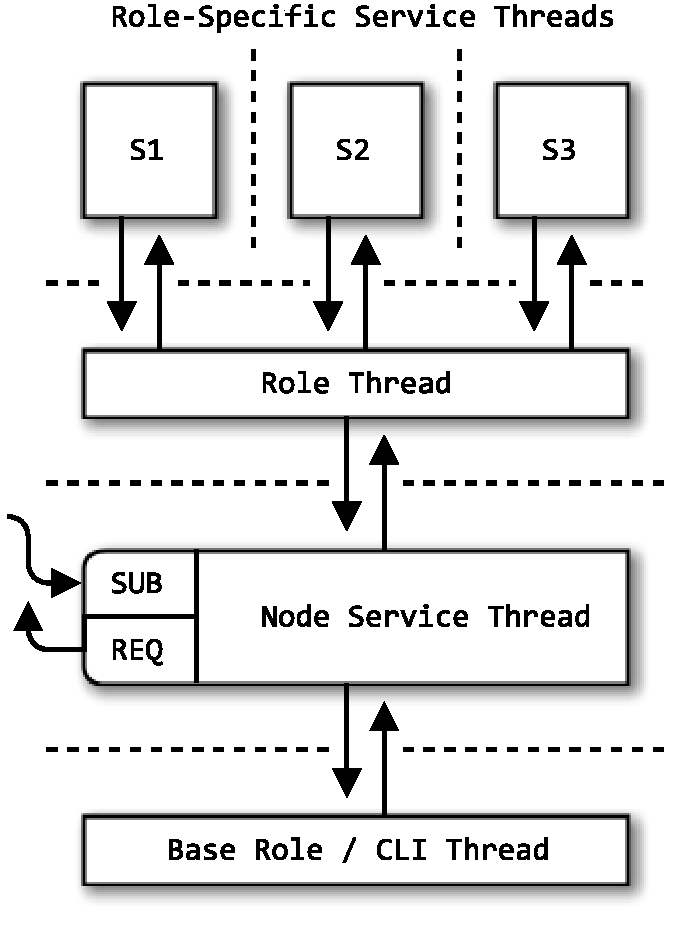
\includegraphics[scale=0.5]{node-role-service.pdf}
    \label{fig:node_role_service_image}
\end{figure}
\end{column}

\begin{column}{5cm}
The \textit{Base} role must be running on each node for it to be part of the \dcamp distributed system. All other roles
are launched from within the \textit{Base} role.
\end{column}

\noi{In this document, a ``\textit{Base} node'' is defined as a \dcamp node which has not yet been configured, i.e. it
     has not joined a running \dcamp system.}
\noi{Node, Role, Services Threading Model Diagram: Thread boundaries are represented by dashed lines. Except for the
     Node service's \texttt{SUB} and \texttt{REQ} sockets, all arrows represent \texttt{PAIR} socket communication.}
\noi{\textit{Base} node can transform into one of the three active \dcamp roles; this transformation is actually the
     \textit{Base} role (via the Node service) launching and managing another role internally.}
\noi{When a \textit{Base} node, only bottom two threads (\textit{Base} and Node) are active.}
\noi{after assignment from the ``discover'' Topology Protocol or CLI, Node service launches an appropriate role thread
     which, in turn, launches one or more role-specific service threads.}
\noi{also various service-to-service communications via \texttt{inproc} sockets (e.g. internal Data Flow Protocol) and
     shared memory (e.g. the Configuration service).}

\end{columns}
\end{frame}

%------------------------------------------------
\subsection{Operation}

%------------
\begin{frame}
\frametitle{Sequence of \dcamp Operation}

\bee[<+->]
\item User promotes a \textit{Root} node via the \dcamp CLI, specifying a configuration file and a \textit{Base} node's
      address.
\item \textit{Root} node connects to each \textit{Base} node and begins the ``discover'' Topology Protocol.
\item \textit{Base} nodes join the \dcamp system at any time, being assigned as \textit{Collector} or \textit{Metric}
      nodes in the topology.
\item \dcamp runs in a steady state, nodes entering or exiting the system at any time.
\item User stops \dcamp by using the \dcamp CLI command.
\item \textit{Root} node begins the ``stop'' Topology Protocol.
\item \textit{Collector} and \textit{Metric} nodes exit the topology and revert to \textit{Base} nodes.
\item \textit{Root} node exits, reverting to \textit{Base} node.
\eee

\noi{\textit{Base} nodes (other \textit{Root}) can be started at any time by using the \dcamp CLI}
\noi{expected \textit{Base} nodes are managed by a watchdog utility}
\end{frame}

%------------
\begin{frame}
\frametitle{Steady-State Operation}
\bee[<+->]
\item Performance counters are sampled, filtered, reported, and logged by the Metric nodes at regular intervals
      according to the \dcamp Configuration.
\item Performance counters received from child nodes are aggregated, filtered, reported, and logged by
      \textit{Collector} nodes at regular intervals according to the \dcamp Configuration.
\item Performance counters received from child nodes are aggregated and logged by \textit{Root} node for later
      processing (e.g. graphing metrics during a test scenario or correlating statistics with a distributed event
      log).
\eee
\end{frame}

%------------------------------------------------
\section{dCAMP Details}
%------------------------------------------------

%------------------------------------------------
\subsection{ZeroMQ Protocols}
\frame{topology}
\frame{configuration}
\frame{data}
\frame{recovery}

%------------------------------------------------
\subsection{Fault Tolerance}
\frame{heartbeating}
\frame{reminder}
\frame{promotion}
\frame{election}

%------------------------------------------------
\section{dCAMP Analysis}
%------------------------------------------------

%------------------------------------------------
\subsection{Transparency}

%------------
\begin{frame}
\frametitle{Strategy}
To measure the impact of \dcamp on a monitored process, a workload is defined and measured with and without \dcamp
active. The measured difference in performance of the monitored process is defined to be \dcampns's monitoring overhead.
\end{frame}

%------------
\begin{frame}
\frametitle{Workload}
Apache JMeter\cite{jmeter} (v2.11) is used to run load against a default-configured Apache instance on a Lenovo Thinkpad
(dual 2.16GHz Centrino Duo T2600, 2GB 667MHz DDR2, SATA) running Ubuntu 13.10. The client machine, a MacBook Pro (2.7GHz
Core i7, 8GB 1333MHz DDR3, SSD) running OSX 10.9, is directly connected to the Apache server via crossover gigabit
Ethernet.

\medskip

Each test run includes 18 different load points, scaling the number of client threads from 2 to 2048. For every load
point, the threads continuously (in this order):

\begin{enumerate}
\item load a static home page,
\item load a PHP page which calculates the 25th Fibonacci number, and
\item download a 5MB file of random binary data.
\end{enumerate}

\noi{Fibonacci workload is CPU-bound, 5MB download is disk-bound, home page workload is only used to seed the client
     connection and is not part of the analysis measurements.}
\noi{After the ramp up phase of each load point (launching 10 threads per second), the test ensures all threads continue
     to execute simultaneously for five minutes before shutting down.}
\noi{The arithmetic mean of the request latency for each step at each load point is then calculated and averaged across
     three distinct runs of the same test.}
\end{frame}

%------------
\begin{frame}
\frametitle{Configuration}

Each \dcamp configuration level monitors four global metrics and three process-specific metrics on the Apache
process(es). The global metrics are CPU usage (\texttt{proc}), memory usage (\texttt{mem}), disk throughput
(\texttt{disk}), and network throughput (\texttt{net}); the Apache metrics are CPU usage (\texttt{apache\_cpu}), memory
usage (\texttt{apache\_mem}), and combined disk/network throughput (\texttt{apache\_io}).

\begin{itemize}
\item \textbf{baseline} -- \dcamp off
\item \textbf{5m} -- all metrics every 300 seconds, heartbeats every 60 seconds
\item \textbf{1m} -- all metrics every 60 seconds, heartbeats every 60 seconds
\item \textbf{10s} -- global metrics every 300 seconds, Apache metrics every 10 seconds, heartbeats every 300 seconds
\item \textbf{1s} -- global metrics every 300 seconds, Apache metrics every 1 second, heartbeats every 300 seconds
\end{itemize}

\noi{No thresholds were defined for any of the configurations. That is, Sensor nodes immediately reported every sample
     instead of holding them for later reporting.}
\end{frame}

%------------
\begin{frame}
\frametitle{CPU-Bound Results}
\centering
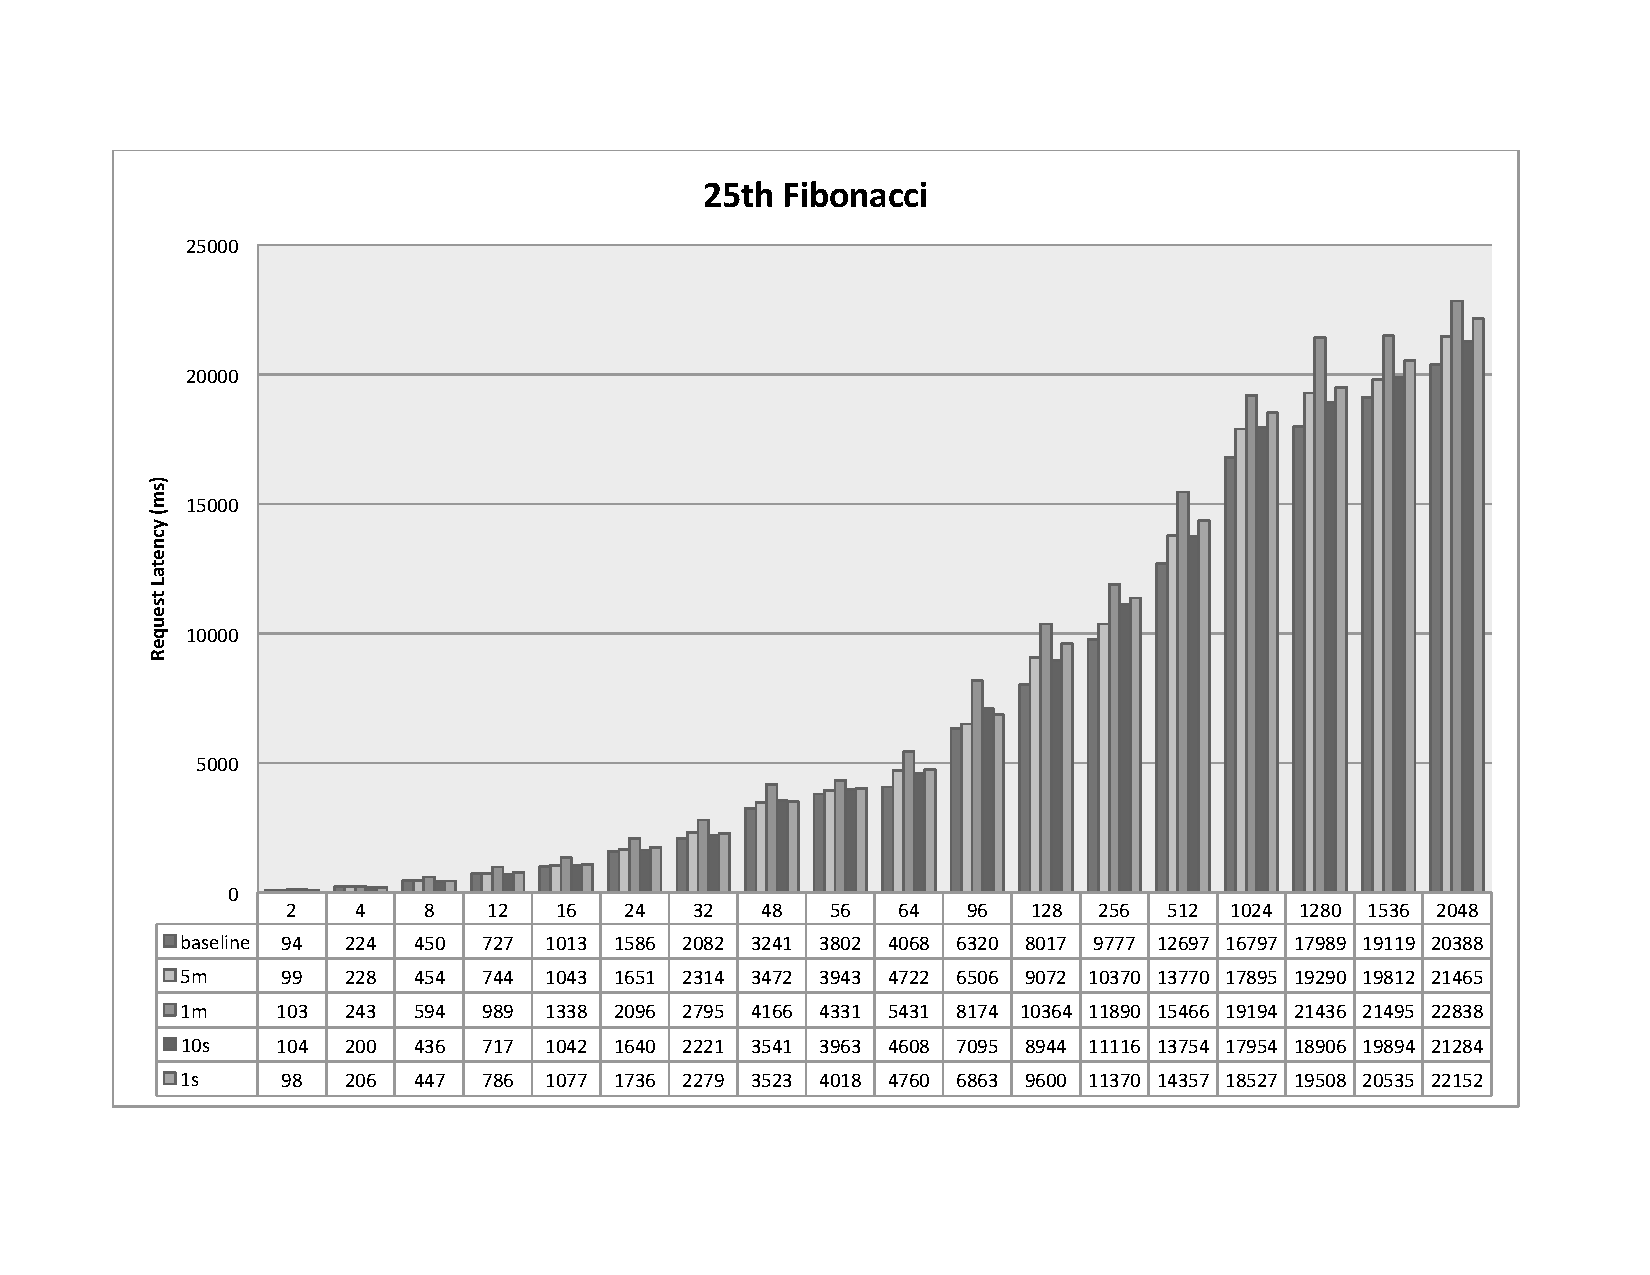
\includegraphics[height=8.6cm,transparent]{compare-fib.pdf}

\noi{In the CPU-bound Fibonacci test, the biggest relative increase in request latency occurs between the runs with two and
four threads. This correlates to the two physical CPU cores on the system exceeding capacity.}
\noi{The 1m config run exhibits the worst performance of all the CPU-bound tests. This shows that global metric monitoring is actually more CPU
intensive than collecting per-process metrics, even for processes with many active processes.}
\noi{The rate at which request latency worsens begins to level off starting at the 512 thread load point. This is also the
load point at which Apache begins to return errors. As the percentage of requests resulting in errors increases, the
latency of the successful requests improves slightly. This explains the trend line shift.}
\end{frame}

%------------
\begin{frame}
\frametitle{Disk-Bound Results}
\centering
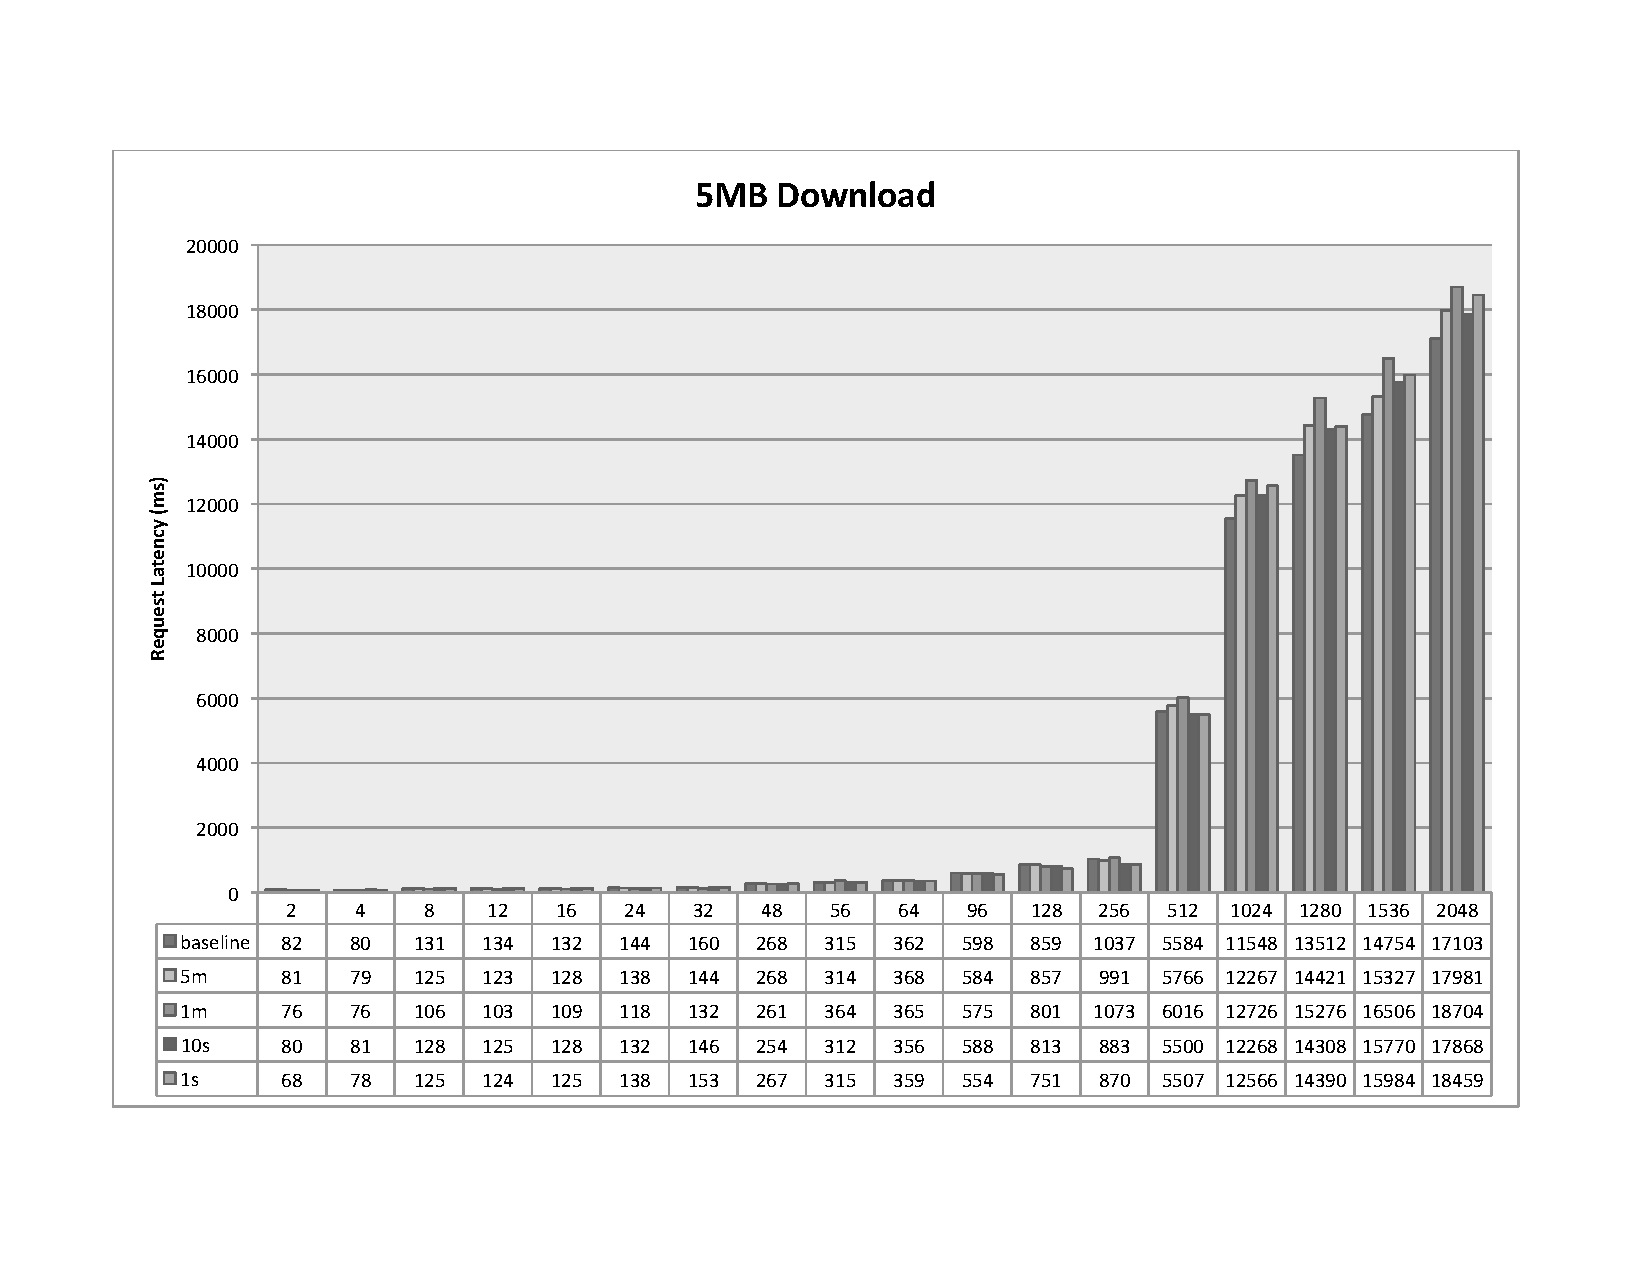
\includegraphics[height=8.6cm,transparent]{compare-down.pdf}

\noi{Apache's disk-bound performance measured in the 5MB download test is relatively unaffected by \dcampns. This is expected
since the infrequent samples being logged to an output file are \dcampns's only disk access.}
\noi{The graph also shows the 512 thread load point as the beginning of a trend line shift, again correlating with the
increase in request error rate.}
\end{frame}

\begin{frame}
\frametitle{Observations}

\bee
\item When nodes are not expected to fail frequently, using longer heartbeat periods reduces the impact \dcamp has on the
system.
\item It is better to monitor a process using a faster sample period than an entire system using a slower sample
period.
\item The \dcamp system impact is noticeable but a considerably smaller factor than the impact hardware limitations
have on performance monitoring.
\item Holding all else constant, slower sample periods have an obviously lower impact on system performance compared
to faster sample periods.
\item Possibly using \dcampns's reporting threshold, system impact can be minimized while still
maintaining fine sample granularity.
\eee

\end{frame}

%------------------------------------------------
\subsection{Scalability}
\frame{workload}
\frame{configuration}
\frame{results}

%------------------------------------------------
\section{Evaluation and Conclusion}
%------------------------------------------------

%------------------------------------------------
\frame{dcamp}

%------------------------------------------------
\frame{contributions}

%------------------------------------------------

%------------
\begin{frame}
\frametitle{References}
\footnotesize{
\begin{thebibliography}{99} % Beamer does not support BibTeX so references must be inserted manually as below

\bibitem{zanikolas2005}[Zanikolas, 2005] {Zanikolas,, Serafeim and Sakellariou,, Rizos} (2005)
\newblock A taxonomy of grid monitoring systems
\newblock \emph{Future Gener. Comput. Syst.} 21(1), 0167-739X, p163--188.

\bibitem{gabel2007}[Gabel, 2007] {Gabel, Mark and Haungs, Michael} (2007)
\newblock {{CAMP}: a common {API} for measuring performance}
\newblock \emph{LISA'07: Proceedings of the 21st conference on Large Installation System Administration Conference}, p1--14

\end{thebibliography}
}
\end{frame}

%----------------------------------------------------------------------------------------
%----------------------------------------------------------------------------------------

\appendix

\section{\appendixname}
\frame{\tableofcontents}

%------------------------------------------------
\subsection{Terminology}

%------------
\begin{frame}
\frametitle{terms}
(page 5-9)
-   perf metric
-   metric sampling, reporting, aggregation, calculation
-   service + role
-   zeromq
-   zeromq address + endpoint
\end{frame}

%------------------------------------------------
\subsection{DPF Evaluation Criterion Details}

%------------
\begin{frame}
\frametitle{Data Delivery Models}
Monitoring information includes fairly static (e.g., software and hardware configuration of a given node) and dynamic
events (e.g., current processor load, memory), which suggests the use of different measurement policies (e.g., periodic
or on demand). In addition, consumer patterns may vary from sparse interactions to long lived subscriptions for
receiving a constant stream of events. In this regard, the monitoring system must support both pull and push data
delivery models.
\end{frame}

%------------
\begin{frame}
\frametitle{Security}
Certain scenarios may require a monitoring service to support security services such as access control, single or mutual
authentication of parties, and secure transport of monitoring information.
\end{frame}

%------------
\begin{frame}
\frametitle{Scalability}
Monitoring systems have to cope efficiently with a growing number of resources, events and users. This scalability can
be achieved as a result of good performance which guarantees that a monitoring system will achieve the needed throughput
within an acceptable response time in a variety of load scenarios.
\end{frame}

%------------
\begin{frame}
\frametitle{Transparency}
Transparency refers to the lack of impact a distributed performance framework makes on the system being monitored. As
\cite{zanikolas2005} states, it is ``typically measured as a function of host (processor, memory, I/O) and network load
(bandwidth) generated by the collection, processing and distribution of events.'' If a framework lacks transparency it
will fail to allow the underlying distributed system to perform well and will produce inaccurate performance
measurements, thereby reducing its Scalability and destroying its Validity.
\end{frame}

%------------
\begin{frame}
\frametitle{Completeness}
The Completeness of a distributed performance framework refers to the exhaustiveness to which it gathers performance
metrics. At a minimum, a framework must provide interfaces for measuring and aggregating performance data about a
system's processor, memory, disk, and network usage. Several distributed performance frameworks provide further detailed
performance metrics about the given distributed system being monitored, but this is usually at the cost of Portability.
\end{frame}

%------------
\begin{frame}
\frametitle{Validity}
A distributed performance framework is only as good as the data is produces; if the sensors or gathering techniques are
inaccurate, then the data is useless at best, misleading at worst. Validity of a framework is achieved when the authors
of a framework provide formal verification of its accuracy.
\end{frame}

%------------
\begin{frame}
\frametitle{Portability}
A framework's ability to run on a completely heterogeneous distributed system without special considerations by the
practitioner is what this work defines as Portability. More specifically, a portable framework has a unified API
regardless of the system architecture, does not restrict itself to applications written in specific programming
languages, and does not require practitioners to manually instrument their application code. This black box
characteristic is vital for a viable distributed performance framework's effectiveness as it allows practitioners to
focus on the performance data and not on a myriad of APIs for various architectures or languages.
\end{frame}

%------------------------------------------------
\subsection{Related Work}
\frame{related work}

%------------------------------------------------
\subsection{ZeroMQ: Sockets and Patterns}
\frame{details}

%------------------------------------------------
\subsection{ZeroMQ: Messaging Patterns}
\frame{Publish/Subscribe}
\frame{Request/Reply}
\frame{Pipeline}
\frame{Exclusive Pair}

%------------------------------------------------
\subsection{dCAMP Messages}
\frame{Topology}
\frame{Configuration}
\frame{Data}

%------------------------------------------------
\subsection{dCAMP Protocols}
\frame{Topology}
\frame{Configuration}
\frame{Branch Recovery}
\frame{Root Recovery}

%------------------------------------------------
\subsection{dCAMP Configuration}
\frame{Node Specification}
\frame{Sample Specification}

%------------------------------------------------
\subsection{dCAMP Metrics}
\frame{overview, dcamp metric groups, pitfall}

\end{document} 
